\title{Other Search-Based Optimization Approaches}
\label{chp:other-search-based-optimization-approaches}
\author{Roberto Santana}
\institute{University of Basque Country}
\maketitle


In previous chapters we have seen detailed examples of search-based optimization algorithms. Here, we present an overview of other search-based techniques. This class of methods can be grouped according to different criteria, among them:

 \begin{itemize}
   \item Single solution versus multiple solutions search-based algorithms.
    %\item Algorithms that use a discrete, continuous or mixed representation.
   \item Black-box versus gray-box optimization algorithms.
    \item Model-less versus model-based algorithms.
 \end{itemize}

 As the name indicates, single-solution search-based algorithms organize the search by maintaining a single solution at each step.   The transitions between solutions can be done according to different criteria.  Examples of single-solution base-search algorithms are the Iterative Descent (or Hill-Climbing) and Simulated Annealing methods presented in previous sections. The difference between Iterative Descent  and Simulated Annealing illustrates that in these algorithms, although a single solution is kept in each iteration,  multiple evaluations might be needed (e.g, a neighborhood of solutions for some variants of Iterative Descent) in order to decide which is the next solution to be selected.

 The best-known family of algorithms that simultaneously uses multiple solutions are population-based evolutionary algorithms such as genetic algorithms (GAs) \cite{Goldberg:1989}. The distinguished  characteristic  of population-based algorithms is that they use selection and recombination operators as a way to identify and exploit partial solutions of high quality (``fitness'') in order to conduct an efficient search of the promising areas of the search space. This goal is more difficult to achieve for search-based methods that use single solutions.  We will we present GAs in more detail in Section~\ref{sec:SINGLE_VS_POP}. 

 Black-box optimization algorithms do not assume the existence of any information about the function or problem being optimized. On the other hand, gray-box optimization methods start from some description of the problem characteristics (e.g., some representation of the problem structure) and use this information to implement specialized and more efficient search operators. Most heuristic optimization methods, including those covered in previous chapters are black-box methods. 


 Model-less optimization methods are those where no global representation of the characteristics or the best solutions or the search progress is created and exploited. They are commonly a choice for problems for which no information is available a-priori. However, in several optimization domains, modeling the characteristics of the promising solutions can contribute to a more efficient search. Model-based search methods are a family of algorithms that implement this approach. Simple GAs  usually apply variation operators on one or two solutions and they are considered model-less methods.  Other evolutionary algorithms apply selection to identify high fitness solutions, but instead of applying mutation and recombination operators, they learn a model that captures the relevant information from the selected solutions. The model is then used to generate or sample new solutions and the steps of selection, modeling and sampling are repeated in each generation. 

 While the three criteria considered in this chapter serve to group optimization algorithms into different classes, a variety of other criteria could be used \cite{Stork_et_al:2020}. The rest of this chapter is organized as follows, Section~\ref{sec:SINGLE_VS_POP} discusses the difference between single-solution and multiple-solutions search-based algorithms using the GA as an example.  A comparison between black-box and gray-box search-based methods is presented in Section~\ref{sec:BLACK_VS_GRAY}. A description of optimization techniques that use modeling of the best solutions is presented in Section~\ref{sec:LESS_VS_MODEL}. Finally, Section~\ref{sec:HPMODEL} provides an example of how to apply different search-based algorithms to the HP protein model, a simple model of protein folding. 


 \section{Single solution versus multiple solutions search-based algorithms} \label{sec:SINGLE_VS_POP}

 Examples of search-based methods that maintain a solution in each iteration, and of population-based algorithms have been presented in previous sections. Here we focus on  GAs  \cite{Goldberg:1989} since they are  one of the most successful optimization methods that have achieved excellent results across a wide range of problem domains. GAs are inspired in the theory of natural selection, e.g., survival of the fittest, and on the application of genetic crossover and mutation operators on a population of candidate solutions.

 Algorithm~\ref{Alg:GA} shows the pseudocode of a simple GA. In Step 1 of the algorithm an initial set of solutions is generated. Usually, these solutions are generated randomly. However, seeding strategies can be applied to start the search from a pool of high-fitness solutions. In Step~3, the solutions are evaluated and subsequently, in Step 4, a subset of solutions is selected according to a predefined selection method. Such method usually gives higher chance to select solutions of better quality. Among the most used strategies for selection are: proportional, tournament, and truncation selection \cite{Blickle_and_Thiele:1996}. 

 In Step~5 of Algorithm~\ref{Alg:GA},  genetic operators are applied on the selected population. These are operators that are used to generate new solutions based on the solutions selected in the previous step.  In the traditional approach, parents chosen from the selected solutions are combined (``mated'') using operators called recombination or crossover operators (e.g., one-point or multiple-point crossover). The offspring then go through another operator called mutation operator (e.g., bit-flip mutation for problems with a binary representation).  While the crossover operator produces new solutions, mutation operators modify single solutions. Finally, in Step~6, the offspring population and the previous population are used to create the new population. This is called ``replacement''.  Among the most used replacement strategies is elitism, a strategy in which the best solution of the previous population is guaranteed to be part of newly generated offspring. As termination criterion a  maximum number of iterations (generations) or some measure of lack of improvement in the solutions are commonly used. 

  \begin{algorithm}[ht!]
  \caption{Simple genetic algorithm}
   
    \begin{algorithmic}[1] 
      \STATE{pop = generate\_population()}

      \REPEAT 
         \STATE  fitness = evaluate\_population(pop)
         \STATE  selected\_pop = select\_solutions(pop, fitness)
         \STATE  offspring = apply\_genetic\_operators(selected\_pop)
         \STATE  pop =  apply\_replacement(pop,offspring)
      \UNTIL Stop criterion is satisfied		
     \end{algorithmic}
	
 \label{Alg:GA}
  \end{algorithm}


  
 One of the reasons that have been used to explain GA's success is the systematic creation and parallel recombination of partial solutions or building blocks \cite{Goldberg:1989}. Considered from that point of view, GAs can be seen as a class of automatic problem decomposition procedures in which information about promising partial solutions is synthesized in multiple ways and refined along generations. However, it has been reported that in many difficult problems blind crossover recombination is not an appropriate choice to exchange information between solutions since partial solutions tend to be disrupted \cite{Watson_et_al:1998}.

 
 % Early analysis of genetic algorithms (GAs) \cite{Goldberg:1989,Holland:1975} based on the building-block hypothesis and the schema theory identified two important issues for successful GA-based optimization. The so-called ``building-block identification'' and ``building-block mixing or exchange'' referred to the need of identifying valuable partial solutions, avoid their disruption, and effectively mix them in the generation of new solutions. GAs that apply simple genetic operators are usually unable to identify the problem variables that interact and therefore they are not very efficient at the time of generating new solutions.  Extensive research has been devoted to design heuristic recombination operators based on a priori information about the problem domain and adaptive genetic operators that attempt to identify and preserve the linkage between the variables. However, these are not general and ro
 
% \subsection{Methods for discrete, continuous and mixed representation}


 \section{Black-box and gray-box search algorithms}   \label{sec:BLACK_VS_GRAY}


 
 Gray-box optimization methods \cite{Chicano_et_2014,Whitley:2015}  develop strategies to solve the optimization problems for which some \emph{a-priori} information is available, notably, those problems with a  ``suitable'' structure. The underlying assumption is that knowing this type of ``structural'' information can not only serve to improve traditional search-based optimization methods, but also to create significantly novel and more efficient approaches.

   Several works assume that the problem structure corresponds to the structure of the  interactions among the problem variables.  For instance, in additively decomposed functions (ADFs) \cite{Muhlenbein_et_al:1999},  the objective function is the  sum of the evaluations of a number of subfunctions defined on subsets of all the variables. If we consider that these subsets of (interacting) variables define the structure of the problem, and this structure is known, then ADFs can be seen as a gray-box optimization problem. Several real-world problems could be included in the class of  gray-box, e.g., MAX-kSAT, Ising model, NK-landscape, etc. \cite{Whitley:2015}.
  
   Even if the difference between black-box and gray-box optimization problems seems sufficiently clear,  there are situations in which information about the problem exists but it is only partial. For instance, we could know which are the groups of related variables where subfunctions are defined, but not the way in which they are related (i.e., the expression for the subfunctions defined in each group).  It is also possible that structural relationships are only known for a limited number of groups, i.e., some definition sets of the function are unknown.  Therefore, for addressing real-world problems a finer grain definition of the type of available problem information  is required.  The information can be: 1) About the structural relationships among variables (definition sets); and  2) About the way in which the interactions are expressed within each group (definition of the subfunctions).  A detailed categorization of optimization problems based on these two criteria is presented in \cite{Santana:2017a}. 

  Taking into account the type of available problem information,  we can describe different types of gray-box search-based optimization methods. For example, \emph{Partition Crossover} is a specialized genetic operator used by some gray-box GAs  \cite{Tinos_et_al:2015,Whitley:2015}. It works by analytically decomposing the  parents into recombining components which, in turn, allows the evaluation function to be decomposed into linearly separable subfunctions during recombination. In \cite{Tinos_et_al:2015}, it was applied to challenging combinatorial problems.   While there are no apparent reasons to set constraints on the structural characteristics  in the general class of gray-box optimization problems, for feasibility and efficiency reasons, gray-box optimizers assume that the  structure of the problem is constrained. For instance, it is assumed that the size of any definition subset of the ADF to be optimized is upper-bounded by a parameter $k$ (e.g.,  \emph{k-bounded pseudo-Boolean} functions as presented in \cite{Whitley:2015}).

  Other population-based optimization algorithms that can be considered as gray-box optimizers are factorized distribution algorithms (FDAs) \cite{Muhlenbein_et_al:1999}. However, they can be also covered under the umbrella of model-based optimization methods and therefore we cover them in the next section. Gray-box optimizers can be also local-search optimizers. In particular, efficient variants of Iterative Descent algorithms have been proposed that exploit the information about the problem structure at the time of exploring the neighborhood of a current solution \cite{Chicano_et_al:2016,Whitley_et_al:2013}.
%Similarly,  combinations of black-box global optimizers and local-search gray-box optimizers have been proposed \cite{Goldman_et_al:2015}. 

 

 \section{Model-less versus model-based algorithms}  \label{sec:LESS_VS_MODEL}


 Model-based search optimizers build a model of the most promising solutions already evaluated by the algorithm and use this model to generate new solutions. The rationale behind this type of algorithm is that the model will be able to capture the patterns shared by multiple high-fitness solutions, and the  methods that generate new solutions from the models, i.e., the sampling methods, will be able to reproduce these patterns in the newly generated solutions.

 
 \begin{algorithm}[ht!]
  \caption{Model-based evolutionary algorithm}
  \begin{algorithmic}[1]
    \STATE{pop = generate\_population()}
      \REPEAT 
         \STATE  fitness = evaluate\_population(pop)
         \STATE  selected\_pop = select\_solutions(pop, fitness)
         \STATE  model = create\_model(selected\_pop)
         \STATE  offspring = sample\_model(model)
         \STATE  pop =  apply\_replacement(pop,offspring)       
       \UNTIL Stop criterion is satisfied		
     \end{algorithmic}
	
 \label{Alg:MEA}
 \end{algorithm}
 
 Algorithm~\ref{Alg:MEA} shows the pseudocode of a typical model-based optimizer. Steps 1-4 and 7 are similar to the simple GA described in Algorithm~\ref{Alg:GA}. The main difference is in the way the selected solutions are used to generate the new population. As previously discussed, in GAs, recombination and mutation operators are applied. In model-based evolutionary algorithms, the model is built from the selected solutions in a first step, and only after the model has been learned, new solutions are sampled from it.

 
 Different types  of models have been used with this type of algorithms, from simple probability models such as histograms \cite{Tsutsui_et_al:2001}, to probabilistic graphical models \cite{Larranaga_et_al:2012}, and  neural networks \cite{Marti_et_al:2008}. Estimation of distribution algorithms (EDAs)  \cite{Muhlenbein_and_Paas:1996r,Larranaga_et_al:2012}, also known as model-building EAs,  are perhaps the most popular family of model-based EAs. They represent the most salient patterns of the selected solutions using a graphical structure that encodes the probabilistic dependencies between the variables, and a set of tables of conditional and marginal probabilities of the variables configurations. The particular choice of the model depends on many factors including the problem representation (e.g., discrete, continuous, mixed) and the number and strength of the problem interactions (when they are known). Typical sampling methods used by EDAs comprise Probabilistic Logic Sampling and Gibbs Sampling \cite{Shakya_and_Santana:2012}.

 While several EDAs learn the graphical structure and the probabilistic tables from data, some algorithms directly derive the model dependencies from  the problem structure. They were originally called factorization-based distribution algorithms (FDAs) \cite{Muhlenbein_et_al:1999} and can be considered as gray-box optimizers. 

 Neural networks have been increasingly applied as models for search-based algorithms \cite{Baluja:2017,Probst_and_Rothlauf:2015}.  In neural networks, information about the problem structure is usually represented by hidden variables or distributed structures. This representation makes interpretability of the model a difficult task. The interpretability of the representation is one important  difference between the way neural networks and probabilistic  graphical models are used in model-based EAs. Another important difference is that neural networks require specific sampling methods that have not been applied to practical optimization problems to the same extent that those used by graphical models. This fact has led to the investigation of new methods for generating new solutions from neural networks \cite{Garciarena_et_al:2020b,Garciarena_et_al:2022}.



\section{Optimization approaches to the HP protein model} \label{sec:HPMODEL}

 A protein can be represented as a sequence of aminoacids. The properties of these aminoacids determine the way the sequence folds into a three-dimensional structure. Hence, an important problem is to predict this structure from the sequence of aminoacids. In this section we illustrate, using a simplified protein model, the way in which some of the search-based methods presented in this chapter can be applied to this problem. 

 \subsection{The hydrophobic-polar (HP) model}

\begin{figure}[htbp]
 \begin{center}
 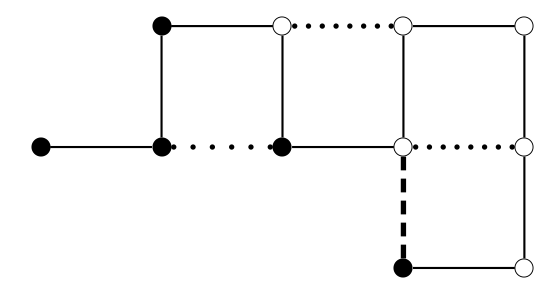
\includegraphics[width=.7\textwidth]{"Part 2 - Search-Based Optimization/Other Search-Based Optimization Approaches/images/HP_Model.png"}
%\begin{pspicture}(0,0)(5.0,5.0)
%\psset{xunit=1.6cm,yunit=1.6cm}
%\dotnode[dotstyle=*,dotscale=2](0,2){A1}
%\dotnode[dotstyle=*,dotscale=2](1,2){A2}
%\dotnode[dotstyle=*,dotscale=2](1,3){A3}
%\dotnode[dotstyle=*,dotscale=2](2,2){A5}
%\dotnode[dotstyle=*,dotscale=2](3,1){A11}
%
%
%\dotnode[dotstyle=o,dotscale=2](2,3){A4}
%\dotnode[dotstyle=o,dotscale=2](3,2){A6}
%\dotnode[dotstyle=o,dotscale=2](3,3){A7}
%\dotnode[dotstyle=o,dotscale=2](4,3){A8}
%\dotnode[dotstyle=o,dotscale=2](4,2){A9}
%\dotnode[dotstyle=o,dotscale=2](4,1){A10}
%
%\ncline{-}{A1}{A2} \ncline{-}{A2}{A3} \ncline{-}{A3}{A4} \ncline{-}{A4}{A5}
%\ncline{-}{A5}{A6} \ncline{-}{A6}{A7} \ncline{-}{A7}{A8} \ncline{-}{A8}{A9}
%\ncline{-}{A9}{A10} \ncline{-}{A10}{A11}
%
%\ncline[linestyle=dotted,dotsep=5pt,linewidth=2.0pt]{-}{A2}{A5}
%\ncline[linestyle=dotted,linewidth=2.0pt]{-}{A6}{A9}
%\ncline[linestyle=dotted,linewidth=2.0pt]{-}{A4}{A7}
%\ncline[linestyle=dashed,linewidth=2.0pt]{-}{A6}{A11}
%\end{pspicture}
 
    \caption{One possible configuration of  sequence  $HHHPHPPPPPH$  in   the HP model. Solid lines indicate a pair of residues neighbors in the sequence. There is   one $HH$ (represented by a dotted line with wide spaces), one $HP$ (represented by a dashed line) and  two $PP$ (represented by dotted lines) contacts.}
 \label{fig:PROTEXAM}
  \end{center}
\end{figure}




The HP protein model considers  hydrophobic (H) residues  and   hydrophilic or polar (P) residues.   In the linear representation of the protein sequence,  hydrophobic residues are represented with the letter H and polar ones with letter P. The structure in which the protein sequence folds is represented as a possible  configuration of the residues  in a regular lattice. For the sake of simplicity, we consider a square lattice.  Given a pair of residues, they are  considered neighbors if they are adjacent  either in the protein chain  (connected neighbors) or in the lattice but not connected in the chain (topological neighbors). Figure~\ref{fig:PROTEXAM} shows the linear representation of an HP instance and one of its possible configurations. 

  An energy function that  measures the interaction  between topological  neighbor residues is defined  as  $\epsilon_{HH}=-1$ and  $\epsilon_{HP}=\epsilon_{PP}=0$. The HP problem consists of  finding a configuration of the sequence in the lattice that is a self-avoided path and minimizes the total energy. The question is then, how to represent a possible configuration (``solution'') of the HP protein sequence. 

  In order to encode a possible 2D configuration of a sequence, we use the relative encoding \cite{Krasnogor_et_al:1999} which specifies the way in which a walk in a lattice is performed. To represent a walk by means of the relative encoding, an $n$-dimensional vector $(X_1,X_2,\dots, X_n)$ is used, where $x_i \in \{0,1,2\}$. Creating a path from a vector starts by locating the two first residues in two (usually fixed) adjacent positions of the lattice. Therefore, although variables $X_1$ and $X_2$ are part of the representation and correspond to the first two residues, they are meaningless for creating the path.

   We can assign an imaginary  direction to the segment that joins the two residues in the lattice, the direction goes from the position of the first residue to the position of the second residue. Following this convention, the next residue of the sequence could be located in three possible positions with respect to this segment: in the position ahead of the segment ($x_i=1$), to the left of this segment  and connected to the last residue ($x_i=0$), or to the right of the segment and connected to the last residue $(x_i=2)$.

  The solution encoding the configuration of the sequence shown in Figure~\ref{fig:PROTEXAM} is $\textbf{x} = (0,0,0,2,2,0,0,2,2,1,2)$. $x_1$ and $x_2$ are arbitrarily set to zero since residues $s_1$ and $s_2$ are always in the same positions. Then, $x_3=0$ indicates that residue $s_3$ will be located  left  to the initial segment formed by the positions of residues $s_1$ and $s_2$, subsequently  $x_4=2$ indicates that residue $s_4$ will be located  right to the segment formed by the locations of residues $s_2$ and $s_3$, and so on.  

 The computation of the HP energy associated to a given solution  $\textbf{x}$ is not straightforward. Firstly,  the configuration has to be constructed simulating the set of movements encoded by the solution. The energy is computed using the interactions that arise in this configuration. The objective function  is the opposite of the energy divided by the number of the sequence's self-intersections.  

 \subsection{Model-based approaches to the HP model}

  The HP model is a focus of research in computational biology  \cite{Gupta_et_al:2005} and  chemical and statistical physics \cite{Kou_et_al:2006,Abe_and_Wako:2006}. It has been addressed using local search optimizers  \cite{Hsu_et_al:2003a} and different variants of evolutionary algorithms  \cite{Unger_and_Moult:1993}. We show here the different approaches that can be applied when considering model-based optimizers, in particular, we focus on EDAs that apply two different classes of models as introduced in \cite{Santana_et_al:2008a}. 

 Once the problem representation has been set, one of the first questions to consider when addressing real-world optimization problems is whether there exists problem information that could be added to the search. This is what gray-box optimizers do.

 For the HP model, we consider two types of information, one is related to the way the 2D configuration is constructed. Since we use a relative representation, it is clear that there is a dependence between the position of residue $i$ and its previous two residues in the sequence. Furthermore, we can expect some  dependence to exist also on its previous $k>2$ residues in the sequence. The other information we know is that some small 2D configurations, where H residues are packed in a small area  contribute more to the energy of the proteins.

 A key question for model-based optimizer is  how to select a model consistent with the interactions of the problem. In the $k$-order Markov model,  the configuration of variable $X_i$ depends on the configuration of the previous $k$ variables, where $k \geq 0$ is a parameter  of the model.  The joint probability distribution of such a model can be factorized as follows:

\begin{equation}
 p_{MK}(\textbf{x}) =  p(x_{1}, \ldots, x_{k+1})  \prod_{i=k+2}^{n}  p( x_{i} \mid  {x_{i-1}, \ldots, x_{i-k}})
\end{equation}
where $p$ represents the marginal and conditional probabilities of the variables. 

This probabilistic model naturally captures the interaction that arises from the relative encoding representation. Notice, that for a given $k$, the structure of the interactions relevant for the model is known before the optimization is conducted.  However, this is not all the information required by an EDA. In order to implement steps 5 and 6 of Algorithm~\ref{Alg:MEA}, it is important to define how the model is learned and sampled. For the  $k$-order Markov model, learning consists of computing the marginal and conditional probability tables for the pre-specified interactions using as data the selected solutions.  To sample a solution, first the unconditioned variables are sampled from the marginal probabilities, and then each conditioned variable is sampled, following the order of the sequence. 


 Another possible approach to the problem is to learn all information about the relevant interactions among the variables directly from the data. A simple model that does this is a tree,  where each variable  may depend on no more than one variable that is called the parent. A probability distribution $p_{Tree}(\textbf{x})$ that is conformal with a tree is defined as:

\begin{equation}
   p_{Tree} (\textbf{x}) =\prod_{i=1}^{n} p(x_i \mid pa(x_i))  \label{eq:T-Tree}
\end{equation}
where $Pa(X_i)$  is the parent of variable $X_i$ in the tree, and $p(x_i \mid pa(x_i))=p(x_i)$ when $Pa(X_i)=\emptyset$, i.e. when $X_i$ is the root of the tree.
%The distribution $p_{Tree}(\textbf{x})$ itself will be called a tree model when no confusion is possible.  Probabilistic trees are represented by acyclic connected graphs.

An EDA that uses a tree model \cite{Baluja_and_Davies:1997} could learn the structure of the model from the analysis of the mutual information between every pair of variables. The model uses the marginal and conditional probability tables determined by the structure. For generating a new solution, first the variable corresponding to the root of the tree is sampled, and then each variable is sampled conditioned on the values of its parent in the tree. 

 \section{Summary and discussion} \label{sec:Summary}


 In this chapter we have presented different classifications of search-based algorithms that use multiple solutions.  We have shown that the decision on whether to apply  black-box or gray-box optimization methods  should depend on the availability of previous information about the optimization problem and the characteristics of this information. Using a-priori knowledge of the problem as part of the search can make optimization more efficient. Similarly, we have presented the main differences between model-less and model-based evolutionary algorithms and illustrated these differences using the simple GA and EDAs as two paradigmatic examples of each type of methods. At the expense of a higher computational cost, model-based search methods can automatically learn characteristics from the most promising solutions, contributing to a more  efficient optimization, and also potentially exploiting and/or unveiling features of the optimization problem. 

 
 


\bibliographystyle{unsrt}
\bibliography{bibliography}
